\section{Interface graphique}
L'utilisateur doit pouvoir interagir avec l'application, il faut donc lui offrir un interface graphique qui lui permette d'effectuer les différentes actions possibles. Cependant si la cible principale est un smartphone cela veut dire que l'espace réservé pour l'interface est restreint. L'idée a été d'avoir quelque chose de léger avec les contrôles sur les bords de l'écran (Figure \ref{fig:ui-normal}).

\begin{figure}[H]
	\centering
	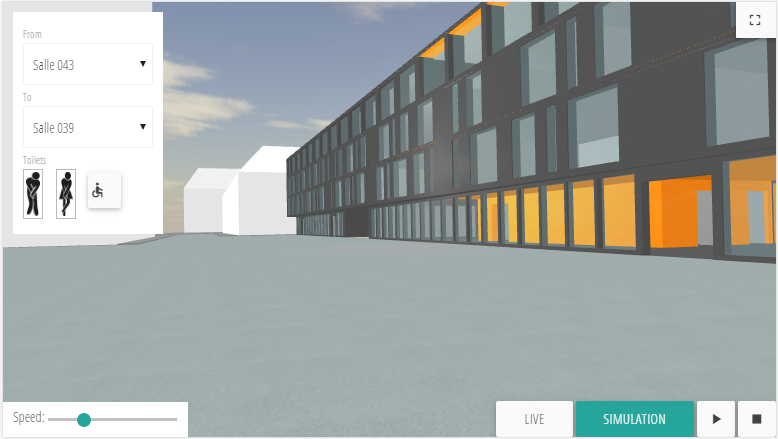
\includegraphics[width=0.9\linewidth]{ui-Normal}
	\caption{Interface graphique d'Arc3D.}
	\label{fig:ui-normal}
\end{figure}

L'interface se compose de cinq zones bien distinctes (références couleurs sur la figure \ref{fig:ui-zones}):
\begin{itemize}
	\item En \emph{rouge}, le choix du trajet ou de la destination. Ainsi que la possibilité d'activer ou non le mode \textit{personnes à mobilité réduite};
	\item En \emph{vert}, un seul bouton qui permet de passer en mode plein écran et d'en revenir;
	\item En \emph{jaune}, un curseur permettant de modifier la vitesse de déplacement;
	\item En \emph{bleu}, deux boutons pour choisir le mode \textit{Live/Simulation} ainsi que deux boutons de mise en marche/pause/arrêt;
	\item Le fond qui est notre canevas WebGL.
\end{itemize}

\begin{figure}[H]
	\centering
	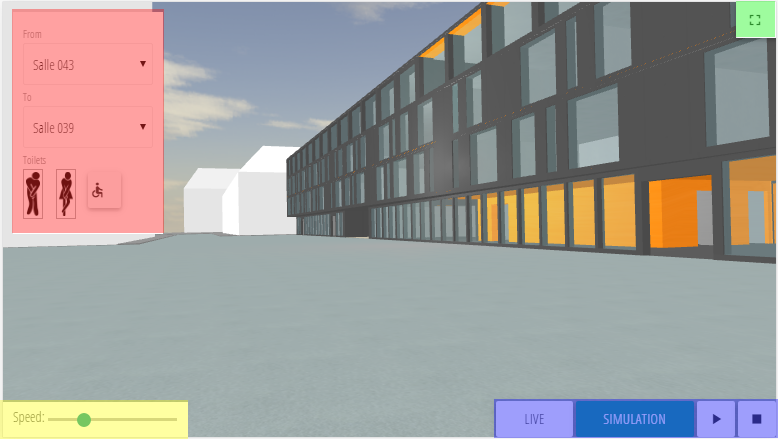
\includegraphics[width=0.9\linewidth]{ui-Zones}
	\caption{Les différentes zones de l'application.}
	\label{fig:ui-zones}
\end{figure}

La dernière fonctionnalité de l'interface n'est pas graphique. Par dessus le canevas WebGL se trouve deux zones cliquables: une à gauche et une à droite (Figure \ref{fig:ui-leftright}). Ces dernières permettent d'effectuer la <<calibration>> du gyroscope à la main. C'est à dire d'ajuster la direction de la caméra dans la scène en décalant respectivement à gauche ou à droite.

\begin{figure}[H]
	\centering
	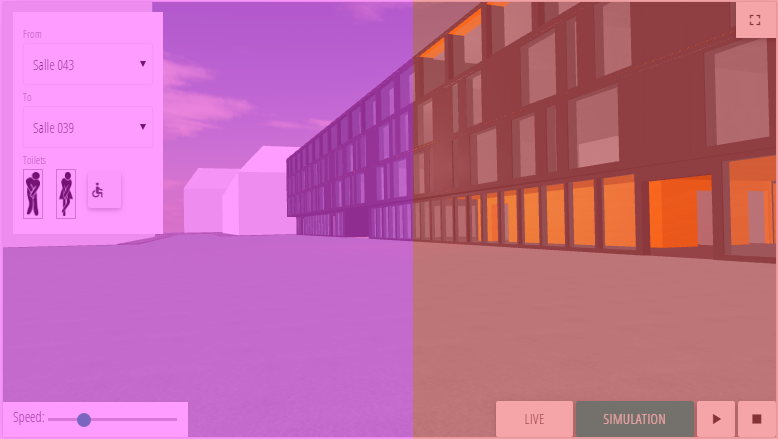
\includegraphics[width=0.9\linewidth]{ui-LeftRight}
	\caption{Les deux zones cliquables qui permettent de décaler la gyroscope.}
	\label{fig:ui-leftright}
\end{figure}